\section{Equilibrium}
When the simulation starts, the system is far from equilibrium due to the random distribution of the velocities of the particle, and the fact that the fcc lattice distribution is not the ground state for a Lennard-Jones potential\cite{travesset2014phase}\cite{van1991can}. To push the system towards equilibrium, the particle velocities are renormalized every 40 timesteps, just as was done in the initialization of the velocities. After each renormalization a jump in the system temperature $T$ towards the desired temperature $T_d$ occurs. This can be seen in Figure \ref{fig:tempequilib}, where the system temperature is plotted during the simulation when the system is still in the equilibration phase. 
\begin{Figure}
 \centering
 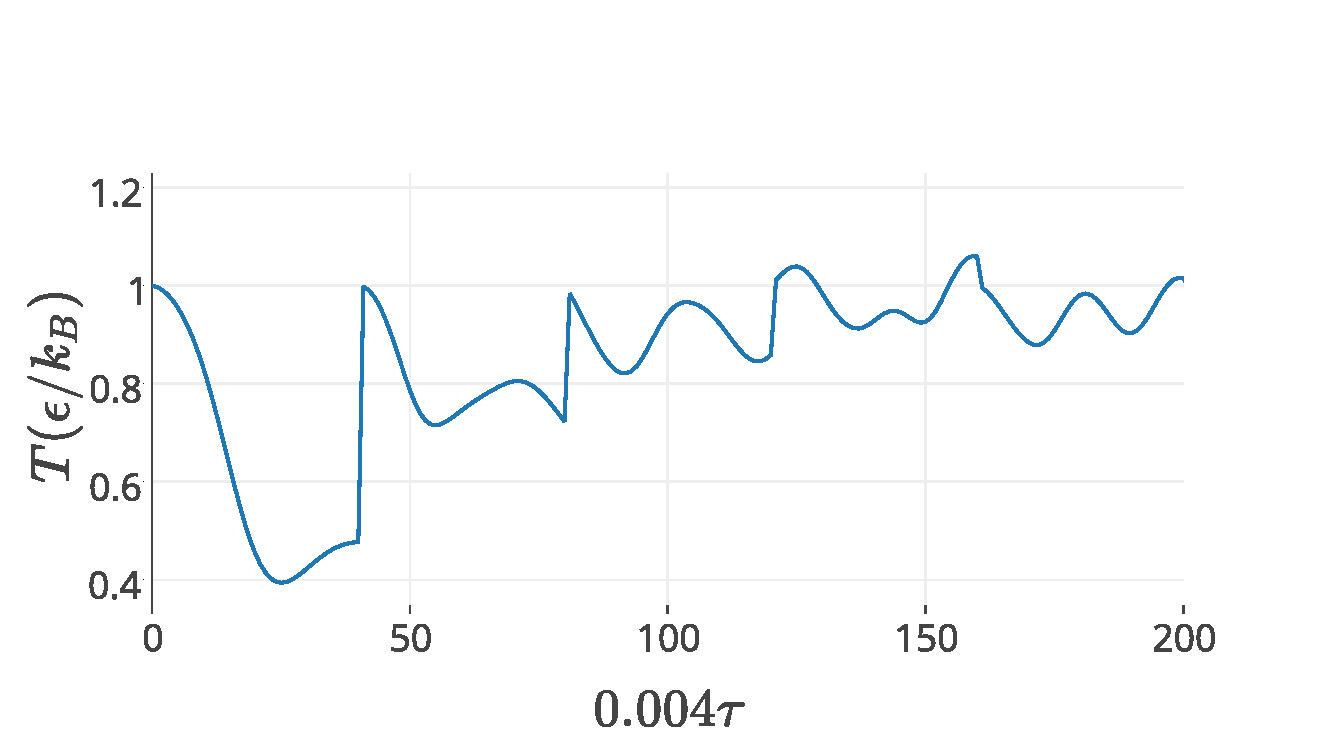
\includegraphics[width=1\linewidth]{equilibration.eps}
 \captionof{figure}{Temperature in equilibration phase. The effects of rescaling can be seen as jumps in $T$, every 40 timesteps.}\label{fig:tempequilib}
\end{Figure}

After 1000 timesteps, the instantaneous temperature remains relatively constant. The system is then assumed to have reached equilibrium. From this point on, physical quantities are calculated.
% A simulation for 108 particles was run, Figure %\ref{fig:instant_temp}
% shows the instantaneous temperature as a function of time steps. The desired temperature was set to 300~K. The temperature fluctuates a lot at the start of the simulation, since the system is far from equilibrium. After around 1000 time steps the system appears to reach equilibrium and the temperature fluctuates around $T_D$. During the equilibration phase the particle velocity is rescaled at intervals of 200 time steps, with the rescaling factor from Eq. \ref{eq:rescale}. Now that the system is in equilibrium, physical quantities can be extracted from the simulation.